\documentclass[compress]{beamer}
\hypersetup{pdfpagemode=FullScreen}
%%
%% Generated by Rodrigo Platte, Arizona State University, May 18 2007 %%
%% Edit this file to change how your presentation looks!
%%
%% For more information, please read the manual: beameruserguide.pdf
%%	 

% Select a theme
%%%%%%%%%%%%%%%%%%%%%%%%%%%
   \usetheme{Frankfurt}
   %\usetheme{Singapore}
%   \usetheme{Madrid}
   %\usetheme{Antibes}
%   \usetheme{Berkeley}
   %\usetheme{default}
%%%%%%%%%%%%%%%%%%%%%%%%%%%

% Select a color theme
%%%%%%%%%%%%%%%%%%%%%%%%%%%
  %\usecolortheme{seagull}
  %\usecolortheme{crane}
  %\usecolortheme{default}
  % \usecolortheme[rgb={.4,0,0}]{structure} % Red colors
    \usecolortheme[rgb={.2,0,0}]{structure} % Dark Red colors
  %\usecolortheme[rgb={.6,.5,.2}]{structure} % Yellow/Green colors
%%%%%%%%%%%%%%%%%%%%%%%%%%%
  
 % Select a font theme
 %%%%%%%%%%%%%%%%%%%%%%%%%%
   %  \usefonttheme{structurebold}
   %  \usefonttheme{structuresmallcapsserif}
   % \usefonttheme{structureitalicserif}
      \usefonttheme{serif}
 %%%%%%%%%%%%%%%%%%%%%%%%%%

 % Select a background color  
 %%%%%%%%%%%%%%%%%%%%%%%%%%%%%%
   %\setbeamertemplate{background canvas}[vertical shading][bottom=white,top=gray!30]
   % \setbeamertemplate{background canvas}[vertical shading][bottom=white,top=red!10!black!30]
   %\setbeamertemplate{background canvas}[vertical shading][bottom=white,top=green!20!black!30]
   % \setbeamertemplate{background canvas}[vertical shading][bottom=white,top=white]
%%%%%%%%%%%%%%%%%%%%%%%%%%%%%%%

% Select a color for math text
%%%%%%%%%%%%%%%%%%%%%%%%%%%%%%% 
% \setbeamercolor{math text}{fg=red!80!black}
%%%%%%%%%%%%%%%%%%%%%%%%%%%%%%%


% This command suppresses the navigation symbols at footline
% comment the command below if you  want navigation symbols 
%\setbeamertemplate{navigation symbols}{}

% Set the size of the font in frame title
\setbeamerfont{frametitle}{size=\normalsize}


% This command will generate a gray footline with the ASU logo in
% each frame
  \useoutertheme{mathASUlogo}


					                                         \usepackage[english]{babel}
\usepackage{graphics}
\usepackage{multimedia} % for movies and sound
\usepackage{times}
\usepackage{tikz}
\usepackage[font=small]{subcaption}
%\usepackage{subcaption}
\captionsetup[sub]{font=small}
\usepackage{stackengine}



\title{The Knife Edge Viscometer}
\author[F. Castillo-Carrasco]{\emph{Francisco Castillo-Carrasco} }
\date{\today}
% Show ASU logo in title page
%%%%%%%%%%%%%%%%%%%%%%
\institute[Mathematics and Statistics]{

\includegraphics[height=.9cm]{ASUlogo.pdf} \\
{\color{ASUred} SCHOOL OF \textbf{MATHEMATICAL AND STATISTICAL SCIENCES}}}
%%%%%%%%%%%%%%%%%%%%%

	%%%%%%%%%%%%%%%%%%%%%%%%%%%%%%%%%%%%%%%%%%
%%%%%%%%%%%% Presentation Starts Here %%%%%%%%%%%%%%%%
	%%%%%%%%%%%%%%%%%%%%%%%%%%%%%%%%%%%%%%%%%%

\begin{document}
%%% Title frame %%%%%
\begin{frame}[plain]
	\titlepage
\end{frame}

%%%%%%%%%%%%%%%%%%%%%%%%%%%%%%%%%%
\begin{frame}
  \frametitle{Outline}
  \tableofcontents[pausesections]
\end{frame}
%%%%%%%%%%%%%%%%%%%%%%%%%%%%%%%%%%

\section[Introduction]{Introduction}

\subsection{The Knife Edge Viscometer}
\begin{frame} \frametitle{The Knife Edge Viscometer}
\begin{figure}
\centering
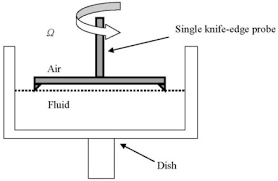
\includegraphics[scale=0.8]{KEviscometer.png}
\end{figure}
\end{frame}

\subsection{Quick Motivation}
\begin{frame} \frametitle{Quick Motivation}
Why do we study this problem?
\begin{itemize}
\item How to measure surface shear viscosity remains a controversial issue.

\item Monomolecular layers are key in broad areas
\begin{itemize}
\item Pharmaceuticals: interfacial processing.
\item Food processing: surfactants.
\item Natural: Gas absorption into a fluid (lungs, oceans).
\end{itemize}
\item Applications where a high degree of mixing is desired (microbioreactors), although at a low level of shear stress.
\end{itemize}
\end{frame}


\subsection{Non-Dimensionalization}
\begin{frame} \frametitle{Non-Dimensionalization}
\begin{columns}
\column{0.5\textwidth}
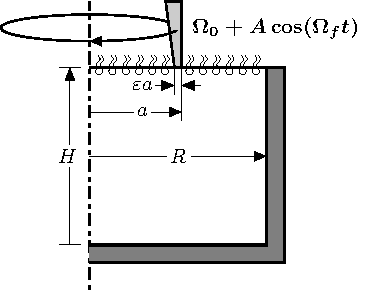
\includegraphics[scale=.8]{scheme.pdf}
\includegraphics[scale=.8]{scheme_ND.pdf}
\column{0.5\textwidth}
\vspace{-8mm}
{\footnotesize
\begin{block}{Using Varialbes $a,\Omega_0, \rho$}
\begin{align*}
A_z &= H/a & A_r &= R/a \\
\alpha &= A/\Omega_0 & \omega_f &= \Omega_f/\Omega_0 \\
\nu &= \mu/\rho & Re &= \nu/a^2\Omega_0 \\
& & Bo &= \mu^s/\mu a \\
\end{align*}
\end{block}}
We have mantained a constant aspect ratio of $A_z = A_r = 2$ .
\end{columns}
\end{frame}


\subsection{Governing Equations}
\begin{frame} \frametitle{Governing Equations (Non-Dimensional)}
\begin{columns}
\column{0.5\textwidth}
\includegraphics[scale=.9]{scheme_ND.pdf}
\column{0.5\textwidth}
\vspace{-8mm}
{\footnotesize
\begin{block}{Cylindrical Coordinates}
$\psi\equiv$ Stream function\\
$\gamma\equiv$ Angular momentum\\
$\eta\equiv$ Azimuthal vorticity
\begin{align*}
\textbf{u} = (u,v,w) &= \left(-\frac{1}{r}\frac{\partial\psi}{\partial z},\frac{\gamma}{r},\frac{1}{r}\frac{\partial\psi}{\partial r}\right)\\
\nabla\times\textbf{u} &= \left(-\frac{1}{r}\frac{\partial\gamma}{\partial z},\eta,\frac{1}{r}\frac{\partial\gamma}{\partial r}\right)
\end{align*}
\vspace{-4mm}
\end{block}}
\end{columns}
\pause
{\small
\vspace{-5mm}
\begin{align*}
\frac{\partial\gamma}{\partial
t}-\frac{1}{r}\frac{\partial\psi}{\partial
z}\frac{\partial\gamma}{\partial
r}+\frac{1}{r}\frac{\partial\psi}{\partial
r}\frac{\partial\gamma}{\partial
z}&=\frac{1}{Re}\left(\frac{\partial^2\gamma}{\partial
z^2}+\frac{\partial^2\gamma}{\partial
r^2}-\frac{1}{r}\frac{\partial\gamma}{\partial
r}\right)\\
\frac{\partial \eta}{\partial t}-\frac{1}{r}\frac{\partial
\psi}{\partial z}\frac{\partial \eta}{\partial
r}+\frac{1}{r}\frac{\partial \psi}{\partial r}\frac{\partial
\eta}{\partial z}+\frac{\eta}{r^2}\frac{\partial \psi}{\partial
z}-\frac{2\gamma}{r^3}\frac{\partial \gamma}{\partial
z}&=\frac{1}{Re}\left(\frac{\partial^2\eta}{\partial
z^2}+\frac{\partial^2\eta}{\partial
r^2}+\frac{1}{r}\frac{\partial\eta}{\partial
r}-\frac{\eta}{r^2}\right)\\
\frac{\partial^2\psi}{\partial z^2}+\frac{\partial^2\psi}{\partial
r^2}-\frac{1}{r}\frac{\partial\psi}{\partial r}&=-r\eta
\end{align*}}
\end{frame}


\subsection{Boundary Conditions}

\begin{frame} \frametitle{Boundary Conditions}
\begin{columns}
\column{0.4\textwidth}
\includegraphics[scale=0.76]{scheme_ND.pdf}
\column{0.6\textwidth}
\pause
\vspace{-6mm}
{\small
\begin{block}{Bottom (no slip)}
\vspace{-5mm}
\begin{align*}
\psi=\gamma=0~\text{ at } z=0\\
\eta=\left.-\frac{1}{r}\frac{\partial^2\psi}{\partial z^2}\right|_{z=0}
\end{align*}
\end{block}}
\pause
\vspace{-1mm}
{\small
\begin{block}{End Wall (no slip)}
\vspace{-5mm}
\begin{align*}
\psi=\gamma=0~\text{ at } r=A_r\\
\eta=\left.-\frac{1}{A_r}\frac{\partial^2\psi}{\partial r^2}\right|_{r=A_r}
\end{align*}
\end{block}}
\pause
\vspace{-1mm}
{\small
\begin{block}{Axis (symmetry)}
\vspace{-5mm}
\begin{align*}
\psi=\gamma=\eta=0~\text{ at } r=0\\
\text{Sure?  }
\left(\left.-\frac{1}{r}\frac{\partial\psi}{\partial r}\right|_{r=0}= 0\right)
\end{align*}
\end{block}}
\end{columns}
\end{frame}


\begin{frame} \frametitle{Boundary Conditions (II)}
\begin{columns}
\vspace{-5mm}
\column{0.7\textwidth}
{\small
\begin{block}{Top (stress balance)}
\vspace{-5mm}
\begin{align*}
\psi=0~\text{ at } z=A_z\\
\eta=\left.-\frac{1}{r}\frac{\partial^2\psi}{\partial z^2}\right|_{z=A_z}\\
\frac{\partial^2 v}{\partial r^2}+\frac{1}{r}\frac{\partial v}{\partial r}-\frac{v}{r^2} = \frac{1}{Bo}\frac{\partial v}{\partial z}~~~~ \forall r\neq A_r/2, z=A_r\\
v=r\left[1+\alpha\cos(\omega_ft)\right] ~~~~ r= A_r/2, z=A_r
\end{align*}
\end{block}}
\column{0.3\textwidth}
$$v = \frac{\gamma}{r}$$
\end{columns}
\pause
{\small
\begin{block}{The limit $Bo\rightarrow\infty$}
\vspace{-4mm}
\begin{align*}
\frac{\partial^2 v}{\partial r^2}+\frac{1}{r}\frac{\partial v}{\partial r}-\frac{v}{r^2} = 0
\end{align*}
The bulk flow and the monolayer are decoupled.
Analytic solution is possible.
\end{block}}

\end{frame}

\section[Results]{Results}

\subsection{Observables}
\begin{frame}\frametitle{Observables}
\begin{columns}
\column{0.4\textwidth}
\begin{block}{Global}
\begin{itemize}
\item Kinetic Energy
\begin{align*}
E_k = \frac{1}{2}\int \|\textbf{u}\|^2dV
\end{align*}
\item Enstrophy
\begin{align*}
E_w = \int \|\nabla\times\textbf{u}\|^2dV
\end{align*}
\item Angular Momentum
\begin{align*}
E_{\gamma} = \int \gamma^2dV
\end{align*}
\end{itemize}
\end{block}
\column{0.4\textwidth}
\begin{block}{Local}
We probe the value of the three velocity components:
\begin{align*}
u &= -\frac{1}{r}\frac{\partial\psi}{\partial z}\\
v &= \frac{\gamma}{r}\\
w &= \frac{1}{r}\frac{\partial\psi}{\partial r}
\end{align*}
 at the point $\left(\frac{3}{4}A_r,\frac{3}{4}A_r\right)$.
\end{block}
\end{columns}
\end{frame}

\subsection{Parameter Sweep}

\begin{frame}\frametitle{Parameter Sweep}
\begin{figure}
\centering
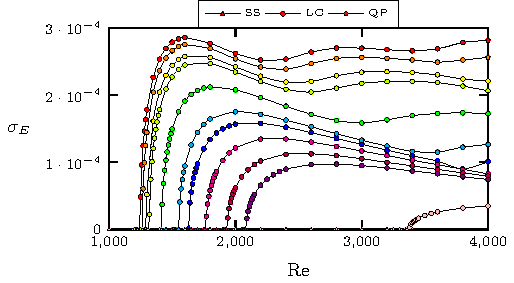
\includegraphics[scale=1.2]{parGraphalpha0e0.pdf}
\end{figure}
\end{frame}

\begin{frame}\frametitle{Scaling}
\begin{figure}
\centering
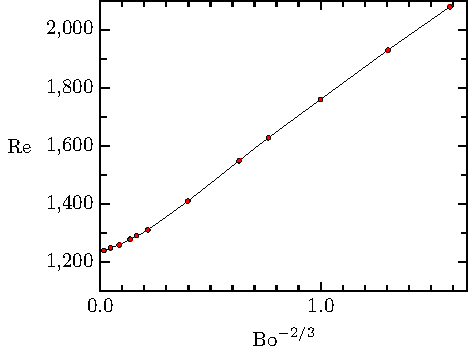
\includegraphics[scale=1]{bifCurveScaled_E.pdf}
\end{figure}
\end{frame}

\subsection{Time-series at the bifurcation}

\begin{frame}\frametitle{At the Hopf Bifurcation}
\vspace{2mm}
{\footnotesize
We now focus on the results for $Bo = 1$ and $Re = 1700$ (right before the bifurcation, $Re_c = 1760$ and $\omega_H = 0.073154$). With this parameters a steady state is reached. We force the system using $\omega = 1+\alpha\cos(\omega_ft)$ using amplitudes $\alpha=0.03,0.05$ and frequencies $\omega_f\in[0.01,0.2]$. 

We plot the standard deviation of the global kinetic energy versus the angular forcing frequency.}
\includegraphics[scale=0.26]{AmpVsFreq_Bo1e0.png}
\end{frame}

\begin{frame}\frametitle{At the Hopf Bifurcation}
\vspace{-2mm}
\includegraphics[scale=0.26]{AmpVsFreq_Bo1e1.png}
\vspace{-2mm}
\includegraphics[scale=0.26]{AmpVsFreq_Bo1e2.png}
\end{frame}

\begin{frame}\frametitle{Time Series $Bo=1$, $Re=1700$, $\alpha=0.05$}
\begin{center}
\begin{figure}
\begin{subfigure}{.2\textwidth}
\centering
\stackunder[5pt]{\includegraphics[scale=0.18]{Ekwf01e-2.png}}{\tiny{$\omega_f = 0.01$}}%
\end{subfigure}
\begin{subfigure}{.2\textwidth}
\centering
\stackunder[5pt]{\includegraphics[scale=0.18]{Ekwf650e-4.png}}{\tiny{$\omega_f = 0.0650$}}%
\end{subfigure}
\begin{subfigure}{.2\textwidth}
\centering
\stackunder[5pt]{\includegraphics[scale=0.18]{Ekwf675e-4.png}}{\tiny{$\omega_f = 0.0675$}}%
\end{subfigure}
\begin{subfigure}{.2\textwidth}
\centering
\stackunder[5pt]{\includegraphics[scale=0.18]{Ekwf700e-4.png}}{\tiny{$\omega_f = 0.0700$}}%
\end{subfigure}
\begin{subfigure}{.2\textwidth}
\centering
\stackunder[5pt]{\includegraphics[scale=0.18]{Ekwf725e-4.png}}{\tiny{$\omega_f = 0.0725$}}%
\end{subfigure}
\begin{subfigure}{.2\textwidth}
\centering
\stackunder[5pt]{\includegraphics[scale=0.18]{Ekwf750e-4.png}}{\tiny{$\omega_f = 0.0750$}}%
\end{subfigure}
\begin{subfigure}{.2\textwidth}
\centering
\stackunder[5pt]{\includegraphics[scale=0.18]{Ekwf775e-4.png}}{\tiny{$\omega_f = 0.0775$}}%
\end{subfigure}
\begin{subfigure}{.2\textwidth}
\centering
\stackunder[5pt]{\includegraphics[scale=0.18]{Ekwf20e-2.png}}{\tiny{$\omega_f = 0.20$}}%
\end{subfigure}
\end{figure}
\end{center}
\end{frame}

\begin{frame}\frametitle{At the Hopf Bifurcation}
To see the time-series, FFTs and orbits go to:
\centering
\vspace{1cm}
\href{https://mathpost.asu.edu/~kiko/Website/research/monitor_alpha3e-2.html}{\beamergotobutton{Results Webpage}}
\end{frame}

%\subsection{Movies}
%\begin{frame}\frametitle{Flow Field Animations}
%\movie[externalviewer]{MOVIES IMPOSSIBLE TO EMBED IN THE BEAMER PRESENTATION}{movie.mp4}
%\end{frame}

\begin{frame}
\centering
\Huge
Thank you.
\end{frame}

\end{document}
